% Canevas et spécimen de thèse.
%
%    \begin{macrocode}
%<*single-template|these-master>
%<<COMMENT
% Document de classe yathesis
%COMMENT
\documentclass{yathesis}
%</single-template|these-master>
%<*these-sample|single-sample>
%<<COMMENT
% Document de classe yathesis, en 12 points, interligne un et demi, et version finale
%COMMENT
\documentclass[12pt,space=onehalf,version=final]{yathesis}
%</these-sample|single-sample>
%<*these-sample|single-sample|single-template|these-master>
%<<COMMENT
%
% Chargement manuel de packages (pas déjà chargés par la classe yathesis)
%COMMENT
\usepackage[utf8]{inputenc}
\usepackage[T1]{fontenc}
\usepackage{kpfonts}
\usepackage{booktabs}
\usepackage{siunitx}
\usepackage{pgfplots}
\usepackage{floatrow}
\usepackage{caption}
\usepackage{microtype}
\usepackage[autostyle]{csquotes}
%<single-sample|these-sample>\usepackage[backend=biber,safeinputenc]{biblatex}
%<single-template|these-master>% \usepackage[backend=biber,safeinputenc]{biblatex}
%</these-sample|single-sample|single-template|these-master>
%<*these-sample|single-sample>
\usepackage{listings}
\usepackage{lipsum} % À proscrire dans un vrai mémoire de thèse !
%</these-sample|single-sample>
%<*single-template|these-master>
%<<COMMENT
% Pour un éventuel glossaire, une liste d'acronymes et/ou une liste de
% symboles
% \usepackage[xindy,acronyms,symbols,toc]{glossaries}
%COMMENT
%</single-template|these-master>
%<*these-sample|single-sample>
\usepackage[xindy,acronyms,symbols,toc]{glossaries}
%</these-sample|single-sample>
%<*single-template|single-sample|these-master|these-sample>
%<<COMMENT
%
% Spécification de la ou des ressources bibliographiques
%COMMENT
%<single-template>% \addbibresource{}
%<single-template>% \addbibresource{}
%<these-master>% \addbibresource{auxiliaires/bibliographie.bib}
%<these-master>% \addbibresource{auxiliaires/}
%<single-sample>\addbibresource{bibliographie.bib}
%<these-sample>\addbibresource{auxiliaires/bibliographie.bib}
%<these-sample|single-sample>\addbibresource{biblatex-examples.bib} % Fournie par biblatex
%<<COMMENT
%
% Génération du glossaire. Facultatif (mais obligatoire si le package
% « glossaries » est chargé).
%COMMENT
%<single-template|these-master>% \makeglossaries
%<these-sample|single-sample>\makeglossaries
%</single-template|single-sample|these-master|these-sample>
%<*single-template|single-sample|these-master|these-sample>
%<<COMMENT
%
% Spécification de la ou des ressources terminologiques. Facultatif.
%COMMENT
%<single-template>% \loadglsentries{}
%<single-template>% \loadglsentries{}
%<single-template>% \loadglsentries{}
%<these-master>% \loadglsentries{auxiliaires/}
%<these-master>% \loadglsentries{auxiliaires/}
%<these-master>% \loadglsentries{auxiliaires/}
%<these-sample>\loadglsentries{auxiliaires/glossaire}
%<these-sample>\loadglsentries{auxiliaires/acronymes}
%<these-sample>\loadglsentries{auxiliaires/symboles}
%</single-template|single-sample|these-master|these-sample>
%<single-sample>% Termes du glossaire
%<*single-sample|glossary-sample>
\newglossaryentry{latex}{%
  name=\LaTeX,%
  description=système de composition de beaux documents%
}
\newglossaryentry{vrnc}{%
  name=langue vernaculaire,%
  plural=langues vernaculaires,%
  description=langue locale parlée au sein d'une communauté%
}
\newglossaryentry{af}{%
  name=ancien français,%
  description= état du français médiéval du \textsc{ix}\ieme{} au
  \textsc{xiii}\ieme{} siècles inclus%
}
\newglossaryentry{mf}{%
  name= moyen français,%
  description= état du français médiéval du \textsc{xiv}\ieme{} au \textsc{xv}\ieme{}
  siècles inclus%
}
%</single-sample|glossary-sample>
%<single-sample>% Acronymes
%<*single-sample|acronyms-sample>
\newacronym{pres}{pres}{Pôle de Recherche et d'Enseignement
  Supérieur}
\newacronym{ulco}{ulco}{Université du Littoral Côte d'Opale}
\newacronym{edspi}{edspi}{École Doctorale Sciences Pour
  l'Ingénieur}
\newacronym{lmpa}{lmpa}{Laboratoire de Mathématiques Pures et
  Appliquées Joseph Liouville}
\newacronym{laser}{laser}{Light Amplification by Stimulated Emission
  of Radiation soit \enquote{amplification de la lumière par
    émission stimulée de rayonnement}}
\newacronym{irm}{irm}{Imagerie par Résonance Magnétique}
\newacronym{rmn}{rmn}{Résonance Magnétique Nucléaire}
\newacronym{ascii}{ascii}{American Standard Code for Information Interchange}
\newacronym{bios}{bios}{Basic Input Output System}
\newacronym{ctan}{ctan}{Comprehensive \TeX{} Archive Network}
\newacronym{dvd}{dvd}{Digital Video Disc}
\newacronym{erp}{erp}{Enterprise Resource Planning}
\newacronym{faq}{faq}{Frequently Asked Questions, traduit en français par
  \enquote{Foire Aux Questions}}
\newacronym{gnu}{gnu}{GNU's Not Unix (acronyme récursif)}
\newacronym{http}{http}{Hypertext Transfer Protocol}
\newacronym{ip}{ip}{Internet Protocol}
\newacronym{jpeg}{jpeg}{Joint Photographic Experts Group}
\newacronym{kdm}{kdm}{KDE Display Manager}
\newacronym{lug}{lug}{Linux Users Group}
\newacronym{mac}{mac}{Medium Access Control}
\newacronym{nfs}{nfs}{Network File System}
\newacronym{ocr}{ocr}{Optical Character Recognition}
\newacronym{p2p}{p2p}{Peer to Peer}
\newacronym{ram}{ram}{Random Access Memory}
\newacronym{radar}{radar}{RAdio Detection And Ranging}
\newacronym{svg}{svg}{Scalable Vector Graphics}
\newacronym{tft}{tft}{Thin-Film Transistor}
\newacronym{utf-8}{utf-8}{Unicode Transformation Format 8 bits}
\newacronym{vga}{vga}{Video Graphics Array}
\newacronym{wpa}{wpa}{Wi-Fi Protected Access}
\newacronym{xhtml}{xhtml}{Extensible HyperText Markup Language}
\newacronym{fsf}{fsf}{Free Software Foundation}
\newacronym{gui}{gui}{Graphical User Interface}
%</single-sample|acronyms-sample>
%<single-sample>% Symboles
%<*single-sample|symbols-sample>
\newglssymbol{ohm}{\si{\ohm}}{ohm}{unité de résistance électrique}
\newglssymbol{exists}{\ensuremath{\exists}}{quantificateur existentiel}{}
\newglssymbol[constanteplanck]{planck}{\ensuremath{h}}{constante de
  Planck}{\ensuremath{h\approx\SI{6,62606957e-34}{J.s}}}
%</single-sample|symbols-sample>
%<*single-template|single-sample|these-master|these-sample>
%<<COMMENT
%
% Génération de l'index. Facultatif.
%COMMENT
%<single-template|these-master>% \makeindex
%<these-sample|single-sample>\makeindex
%</single-template|single-sample|these-master|these-sample>
%<*these-sample|these-master>
%<<COMMENT
%
% Les réglages figurant habituellement dans le préambule, notamment concernant
% la bibliographie et les éventuels glossaires et index, peuvent être saisis
% dans le fichier « thesis.cfg » (situé dans le sous-dossier « configuration »)
% qui est automatiquement importé par la classe yathesis.
%COMMENT
%</these-sample|these-master>
%<*cfg-master|cfg-sample>
%<<COMMENT
%%%%%%%%%%%%%%%%%%%%%%%%%%%%%%%%%%%%%%%%%%%%%%%%%%%%%%%%%%%%%%%%%%%%%%%%%%%%%%%
% Ce fichier doit s'appeler « thesis.cfg » et se situer dans le dossier
% « configuration » ; sinon, la classe yathesis ne le détectera pas.
%%%%%%%%%%%%%%%%%%%%%%%%%%%%%%%%%%%%%%%%%%%%%%%%%%%%%%%%%%%%%%%%%%%%%%%%%%%%%%%
%COMMENT
%</cfg-master|cfg-sample>
%<*single-template|single-sample|cfg-master|cfg-sample>
%<<COMMENT
%
% Configuration des styles du glossaire et de la liste
% d'acronymes. Facultatif.
%COMMENT
%<single-template|cfg-master>% \setglossarystyle{}
%<single-template|cfg-master>% \setacronymstyle{}
%<cfg-sample|single-sample>\setglossarystyle{indexhypergroup}
%<cfg-sample|single-sample>\setacronymstyle{long-sc-short}
%<*cfg-sample|single-sample>
%<<COMMENT
%
% Configuration globale de l'apparence des listings informatiques
%COMMENT
\lstset{%
  language=C,
  numbers=left,
  frame=leftline,
  framerule=0.8pt,
  rulecolor=\color{red},
  basicstyle=\ttfamily,
  keywordstyle=\color{blue}\bfseries,
  stringstyle=\color{cyan},
  commentstyle=\color{gray}\itshape
}
%<<COMMENT
%
% Les figures flottantes et leurs légendes sont dans un (même) cadre
%COMMENT
\floatsetup[figure]{style=BOXED}%
%<<COMMENT
%
% Numéro de version du package pgfplots
%COMMENT
\pgfplotsset{compat=1.10}
%<<COMMENT
%
% Ajustement pour éviter, dans la table des matières, des débordements de
% numéros de pages dans la marge de droite
%COMMENT
\makeatletter
\renewcommand*\@pnumwidth{29pt}
\makeatother
%<<COMMENT
%COMMENT
%</cfg-sample|single-sample>
%</single-template|single-sample|cfg-master|cfg-sample>
%<*single-sample|these-sample|these-master>
%<<COMMENT
%
%COMMENT
%<these-sample|these-master>% Importation manuelle du fichier de macros personnelles
%<!single-sample>

%</single-sample|these-sample|these-master>
%<*macros-master>
%</macros-master>
%<*single-sample|macros-sample>
%<<COMMENT
% Macro pour mettre en forme les noms de fichiers
%COMMENT
\newcommand\fichier[1]{\texttt{#1}}
%<<COMMENT
% Macro pour mettre en forme les noms de packages LaTeX
%COMMENT
\newcommand\package[1]{\textsf{#1}}
%<<COMMENT
% Macro pour mettre en forme des locutions étrangères
%COMMENT
\newcommand{\locution}[1]{\emph{#1}}
%</single-sample|macros-sample>
%<*these-sample|single-sample>
%<<COMMENT
%
% Commande permettant de faire figurer d'un seul coup toutes les références des
% ressources bibliographiques ci-dessus, même si elles ne sont pas citées
% explicitement (à proscrire dans un vrai mémoire de thèse !)
%COMMENT
\nocite{*}
%</these-sample|single-sample>
%<*these-sample|single-sample|single-template|these-master>
%<<COMMENT
%
%%%%%%%%%%%%%%%%%%%%%%%%%%%%%%%%%%%%%%%%%%%%%%%%%%%%%%%%%%%%%%%%%%%%%%%%%%%%%%%
%%%%%%%%%%%%%%%%%%%%%%%%%%%%%%%%%%%%%%%%%%%%%%%%%%%%%%%%%%%%%%%%%%%%%%%%%%%%%%%
% Début du document
%%%%%%%%%%%%%%%%%%%%%%%%%%%%%%%%%%%%%%%%%%%%%%%%%%%%%%%%%%%%%%%%%%%%%%%%%%%%%%%
%%%%%%%%%%%%%%%%%%%%%%%%%%%%%%%%%%%%%%%%%%%%%%%%%%%%%%%%%%%%%%%%%%%%%%%%%%%%%%%
%COMMENT
\begin{document}
%<<COMMENT
%
%%%%%%%%%%%%%%%%%%%%%%%%%%%%%%%%%%%%%%%%%%%%%%%%%%%%%%%%%%%%%%%%%%%%%%%%%%%%%%%
% Caractéristiques du document
%%%%%%%%%%%%%%%%%%%%%%%%%%%%%%%%%%%%%%%%%%%%%%%%%%%%%%%%%%%%%%%%%%%%%%%%%%%%%%%
%
% Préparation des pages de couverture et de titre
%%%%%%%%%%%%%%%%%%%%%%%%%%%%%%%%%%%%%%%%%%%%%%%%%%%%%%%%%%%%%%%%%%%%%%%%%%%%%%%
%COMMENT
%</these-sample|single-sample|single-template|these-master>
%<*these-sample|these-master>
%<<COMMENT
% Les caractéristiques de la thèse sont saisies dans le fichier
% « characteristics.tex » (situé dans le dossier « configuration »).
%COMMENT
%</these-sample|these-master>
%<*single-template|single-sample|characteristics-sample|characteristics-master>
%<<COMMENT
% Auteur de la thèse : prénom (1er argument obligatoire), nom (2e argument
% obligatoire) et éventuel courriel (argument optionnel). Les éventuels accents
% devront figurer et le nom /ne/ doit /pas/ être saisi en capitales.
%COMMENT
%<single-template|characteristics-master>\author[]{}{}
%<characteristics-sample|single-sample>\author[aa@zygo.fr]{Alphonse}{Allais}
%<<COMMENT
%
% Titre de la thèse dans la langue principale (argument obligatoire) et dans la
% langue secondaire (argument optionnel).
%COMMENT
%<single-template|characteristics-master>\title[]{}
%<characteristics-sample|single-sample>\title[Laugh's Chaos]{Le chaos du rire}
%<<COMMENT
%
% Sous-titre de la thèse dans la langue principale (argument obligatoire) et
% dans la langue secondaire (argument optionnel). Facultatif.
%COMMENT
%<single-template|characteristics-master>% \subtitle[]{}
%<characteristics-sample|single-sample>\subtitle[Chaos' laugh]{Le rire du chaos}
%<<COMMENT
%
% Champ disciplinaire dans la langue principale (argument obligatoire) et dans
% la langue secondaire (argument optionnel).
%COMMENT
%<single-template|characteristics-master>\academicfield[]{}
%<characteristics-sample|single-sample>\academicfield[Mathematics]{Mathématiques}
%<<COMMENT
%
% Spécialité dans la langue principale (argument obligatoire) et dans la langue
% secondaire (argument optionnel). Facultatif.
%COMMENT
%<single-template|characteristics-master>\speciality[]{}
%<characteristics-sample|single-sample>\speciality[Dynamical systems]{Systèmes dynamiques}
%<<COMMENT
%
% Date de la soutenance, au format {jour}{mois}{année} donnés sous forme de
% nombres.
%COMMENT
%<single-template|characteristics-master>\date{}{}{}
%<characteristics-sample|single-sample>\date{1}{1}{2015}
%<<COMMENT
%
% Sujet pour les méta-données du PDF. Facultatif.
%COMMENT
%<single-template|characteristics-master>\subject[]{}
%<characteristics-sample|single-sample>\subject[Chaotic Laugh]{Rire chaotique}
%<<COMMENT
%
% Nom (argument obligatoire) du PRES. Facultatif.
%COMMENT
%<single-template|characteristics-master>\pres[logo=,url=]{}
%<characteristics-sample>\pres[logo=images/pres]{Université Lille Nord de France}
%<single-sample>\pres[logo=pres]{Université Lille Nord de France}
%<<COMMENT
%
% Nom (argument obligatoire) de l'institut (principal en cas de cotutelle).
%COMMENT
%<single-template|characteristics-master>\institute[logo=,url=]{}
%<characteristics-sample>\institute[logo=images/ulco,url=http://www.univ-littoral.fr/]{ULCO}
%<single-sample>\institute[logo=ulco,url=http://www.univ-littoral.fr/]{ULCO}
%<<COMMENT
%
% En cas de cotutelle (normalement, seulement dans le cas de cotutelle
% internationale), nom (argument obligatoire) du second institut. Facultatif.
%COMMENT
%<single-template|characteristics-master>% \coinstitute[logo=]{}
%<characteristics-sample>\coinstitute[logo=images/paris13,url=http://www.univ-paris13.fr/]{Université de Paris~13}
%<single-sample>\coinstitute[logo=paris13,url=http://www.univ-paris13.fr/]{Université de Paris~13}
%<<COMMENT
%
% Nom (argument obligatoire) de l'école doctorale. Facultatif.
%COMMENT
%<single-template|characteristics-master>\doctoralschool[url=]{}
%<characteristics-sample|single-sample>\doctoralschool[url=http://edspi.univ-lille1.fr/]{ED Régionale SPI 72}
%<<COMMENT
%
% Nom (1er argument obligatoire) et adresse (2e argument obligatoire) du
% laboratoire (ou de l'unité) où la thèse a été préparée, à utiliser /autant de
% fois que nécessaire/.
%COMMENT
\laboratory[
%<single-template|characteristics-master>logo=,
%<single-template|characteristics-master>telephone=,
%<single-template|characteristics-master>fax=,
%<single-template|characteristics-master>email=,
%<single-template|characteristics-master>url=
%<single-template|characteristics-master>]{}{%
%<single-template|characteristics-master>  \\
%<single-template|characteristics-master>  \\
%<single-template|characteristics-master>  \\
%<single-template|characteristics-master>  \\
%<single-template|characteristics-master>  \\
%<single-template|characteristics-master>  }
%<characteristics-sample>logo=images/labo,
%<single-sample>logo=labo,
%<characteristics-sample|single-sample>logoheight=1.25cm,
%<characteristics-sample|single-sample>telephone=(33)(0)3 21 46 55 86,
%<characteristics-sample|single-sample>fax=(33)(0)3 21 46 55 75,
%<characteristics-sample|single-sample>email=secretariat@lmpa.univ-littoral.fr,
%<characteristics-sample|single-sample>url=http://www-lmpa.univ-littoral.fr/
%<characteristics-sample|single-sample>]{LMPA Joseph Liouville}{%
%<characteristics-sample|single-sample>  Maison de la Recherche Blaise Pascal \\
%<characteristics-sample|single-sample>  50, rue Ferdinand Buisson            \\
%<characteristics-sample|single-sample>  CS 80699                             \\
%<characteristics-sample|single-sample>  62228 Calais Cedex                   \\
%<characteristics-sample|single-sample>  France}
%<<COMMENT
%
% Directeur(s) de thèse et membres du jury, saisis au moyen des commandes
% \supervisor, \cosupervisor, \comonitor, \referee, \committeepresident,
% \examiner, \guest, à utiliser /autant de fois que nécessaire/ et /seulement
% si nécessaire/. Toutes basées sur le même modèle, ces commandes ont
% 2 arguments obligatoires, successivement les prénom et nom de chaque
% personne. Si besoin est, on peut apporter certaines précisions en argument
% optionnel, essentiellement au moyen des clés suivantes :
% - « professor », « seniorresearcher », « mcf », « mcf* »,
%   « juniorresearcher », « juniorresearcher* » (qui peuvent ne pas prendre de
%   valeur) pour stipuler le corps auquel appartient la personne ;
% - « affiliation » pour stipuler l'institut auquel est affiliée la personne ;
% - « female » pour stipuler que la personne est une femme pour que certains
%   mots clés soient accordés en genre.
%
%COMMENT
%<single-template|characteristics-master>\supervisor[,affiliation=]{}{}
%<characteristics-sample|single-sample>\supervisor[professor,affiliation=ULCO]{Michel}{de Montaigne}
%<single-template|characteristics-master>% \cosupervisor[,affiliation=]{}{}
%<characteristics-sample|single-sample>\cosupervisor[mcf*,affiliation=ULCO]{Charles}{Baudelaire}
%<single-template|characteristics-master>% \comonitor[,affiliation=]{}{}
%<characteristics-sample|single-sample>\comonitor[mcf,affiliation=ULCO]{Étienne}{de la Boétie}
%<single-template|characteristics-master>\referee[,affiliation=]{}{}
%<characteristics-sample|single-sample>\referee[professor,affiliation=IHP]{René}{Descartes}
%<single-template|characteristics-master>\referee[,affiliation=]{}{}
%<characteristics-sample|single-sample>\referee[seniorresearcher,affiliation=CNRS]{Denis}{Diderot}
%<single-template|characteristics-master>\committeepresident[,affiliation=]{}{}
%<characteristics-sample|single-sample>\committeepresident[professor,affiliation=ENS Lyon]{Victor}{Hugo}
%<single-template|characteristics-master>\examiner[,affiliation=]{}{}
%<characteristics-sample|single-sample>\examiner[mcf,affiliation=Université de Paris~13]{Sophie}{Germain}
%<single-template|characteristics-master>\examiner[,affiliation=]{}{}
%<characteristics-sample|single-sample>\examiner[juniorresearcher,affiliation=INRIA]{Joseph}{Fourier}
%<single-template|characteristics-master>\examiner[,affiliation=]{}{}
%<characteristics-sample|single-sample>\examiner[juniorresearcher*,affiliation=CNRS]{Paul}{Verlaine}
%<single-template|characteristics-master>% \guest{}{}
%<characteristics-sample|single-sample>\guest{George}{Sand}
%<<COMMENT
%
% Mention du numéro d'ordre de la thèse (s'il est connu, ce numéro est
% à spécifier en argument optionnel). Facultatif.
%COMMENT
%<single-template|characteristics-master>% \ordernumber[]
%<characteristics-sample|single-sample>\ordernumber[42]
%<<COMMENT
%
% Préparation des mots clés dans la langue principale (1er argument) et dans la
% langue secondaire (2e argument)
%%%%%%%%%%%%%%%%%%%%%%%%%%%%%%%%%%%%%%%%%%%%%%%%%%%%%%%%%%%%%%%%%%%%%%%%%%%%%%%
%COMMENT
%<single-template|characteristics-master>\keywords{}{}
%<characteristics-sample|single-sample>\keywords{chaos, rire}{chaos, laugh}
%</single-template|single-sample|characteristics-sample|characteristics-master>
%<*these-sample|single-template|single-sample|these-master>
%<<COMMENT
%
% Production des pages de couverture et de titre
%%%%%%%%%%%%%%%%%%%%%%%%%%%%%%%%%%%%%%%%%%%%%%%%%%%%%%%%%%%%%%%%%%%%%%%%%%%%%%%
%COMMENT
\maketitle
%<<COMMENT
%
%%%%%%%%%%%%%%%%%%%%%%%%%%%%%%%%%%%%%%%%%%%%%%%%%%%%%%%%%%%%%%%%%%%%%%%%%%%%%%%
% Début de la partie liminaire de la thèse
%%%%%%%%%%%%%%%%%%%%%%%%%%%%%%%%%%%%%%%%%%%%%%%%%%%%%%%%%%%%%%%%%%%%%%%%%%%%%%%
%
% Production de la page de clause de non-responsabilité. Facultatif.
%COMMENT
\makedisclaimer
%<<COMMENT
%
% Production de la page de mots clés. Facultatif.
%COMMENT
\makekeywords
%<<COMMENT
%
% Production de la page affichant les logo, nom et coordonnées du ou des
% laboratoires (ou unités de recherche) où la thèse a été
% préparée. Facultatif.
%COMMENT
\makelaboratory
%<<COMMENT
%
% Dédicace(s). Facultatif.
%COMMENT
%<these-sample|these-master>% Dédicace(s)
\dedication{Je dédie ce travail\\à tous ceux qui le méritent}
\dedication{À mon directeur bien-aimé !}
\dedication{À mon co-directeur bien-co-aimé !}
% Production de la page de dédicace(s)
\makededications


%</these-sample|single-template|single-sample|these-master>
%<*single-template|single-sample|dedications-sample|dedications-master>
%<dedications-sample|dedications-master>% Dédicace(s).
%<single-template|dedications-master>\dedication{}
%<single-template|dedications-master>\dedication{}
%<dedications-sample|single-sample>\dedication{Je dédie ce travail\\à tous ceux qui le méritent}
%<dedications-sample|single-sample>\dedication{À mon directeur bien-aimé !}
%<dedications-sample|single-sample>\dedication{À mon co-directeur bien-co-aimé !}
%<dedications-sample|dedications-master>% Production de la page de dédicace(s).
%<single-template|single-sample>% Production de la page de dédicace(s). Facultatif.
\makededications
%</single-template|single-sample|dedications-sample|dedications-master>
%<*these-sample|single-sample|single-template|these-master>
%<<COMMENT
%
% Épigraphe(s). Facultatif.
%COMMENT
%<these-sample|these-master>% Épigraphes(s).
\frontepigraph{}{}
\frontepigraph{}{}
% Production de la page de d'épigraphe(s).
\makefrontepigraphs

%</these-sample|single-sample|single-template|these-master>
%<*single-template|single-sample|epigraphs-sample|epigraphs-master>
%<epigraphs-sample|epigraphs-master>% Épigraphes(s).
%<single-template|epigraphs-master>\frontepigraph{}{}
%<single-template|epigraphs-master>\frontepigraph{}{}
%<single-sample|epigraphs-sample>\frontepigraph{Science sans conscience n'est que ruine de l'âme.}{François Rabelais}
%<single-sample|epigraphs-sample>\frontepigraph[english]{I can resist everything, except temptation!}{Oscar Wilde}
%<single-sample|epigraphs-sample>\frontepigraph{Il est plus facile de désintégrer un atome qu'un préjugé.}{Albert Einstein}
%<epigraphs-sample|epigraphs-master>% Production de la page de d'épigraphe(s).
%<single-template|single-sample>% Production de la page de d'épigraphe(s). Facultatif.
\makefrontepigraphs
%</single-template|single-sample|epigraphs-sample|epigraphs-master>
%<*single-template|single-sample|abstract-sample|abstract-master>
%<single-template|single-sample>%
%<<COMMENT
% Résumés (de 1700 caractères maximum, espaces compris) dans la
% langue principale (1re occurrence de l'environnement « abstract »)
% et, facultativement, dans la langue secondaire (2e occurrence de
% l'environnement « abstract »).
%COMMENT
\begin{abstract}
%<single-template|abstract-master>% ...
%<single-sample|abstract-sample>  \lipsum[1-2]
\end{abstract}
\begin{abstract}
%<single-template|abstract-master>% ...
%<single-sample|abstract-sample>  \lipsum[3-4]
\end{abstract}
%<<COMMENT
%
% Production de la page de résumés.
%COMMENT
\makeabstract
%</single-template|single-sample|abstract-sample|abstract-master>
%<*these-sample|these-master>
%<<COMMENT
%
% Résumés succincts.
%COMMENT
% Résumés (de 1700 caractères maximum, espaces compris) dans la
% langue principale (1re occurrence de l'environnement « abstract »)
% et, facultativement, dans la langue secondaire (2e occurrence de
% l'environnement « abstract ») :
\begin{abstract}
  \lipsum[1-2]
\end{abstract}
\begin{abstract}
  \lipsum[3-4]
\end{abstract}
%
% Production de la page de résumés :
\makeabstract

%</these-sample|these-master>
%<*these-sample|single-template|single-sample|these-master>
%<<COMMENT
%
% Chapitre de remerciements. Facultatif.
%COMMENT
%<these-sample|these-master>\acknowledgements

%</these-sample|single-template|single-sample|these-master>
%<*single-template|single-sample|acknowledgments-sample|acknowledgments-master>
\chapter{Remerciements}
%<single-template|acknowledgments-master>% ...
%<acknowledgments-sample|single-sample>\section{Une section de remerciements}
%<acknowledgments-sample|single-sample>\lipsum[1]
%<acknowledgments-sample|single-sample>\section{Une autre section de remerciements}
%<acknowledgments-sample|single-sample>\lipsum[2-9]
%</single-template|single-sample|acknowledgments-sample|acknowledgments-master>
%<*these-sample|single-template|single-sample|these-master>
%<<COMMENT
%
% Chapitre d'avertissement. Facultatif.
%COMMENT
%<these-master>% \chapter{Avertissement}
Thèse hilarante, comme le gaz du même nom !

%<these-sample>\chapter{Avertissement}
Thèse hilarante, comme le gaz du même nom !

%</these-sample|single-template|single-sample|these-master>
%<*single-template|caution-sample|single-sample|caution-master>
%<single-template|caution-master>% \chapter{Avertissement}
%<caution-sample|single-sample>\chapter{Avertissement}
%<single-template|caution-master>% ...
%<caution-sample|single-sample>Thèse hilarante, comme le gaz du même nom !
%</single-template|caution-sample|single-sample|caution-master>
%<*these-sample|single-sample|single-template|these-master>
%<<COMMENT
%
% Liste des acronymes. Facultatif.
%COMMENT
%<single-template|these-master>% \printacronyms
%<these-sample|single-sample>\printacronyms
%<<COMMENT
%
% Liste des symboles. Facultatif.
%COMMENT
%<single-template|these-master>% \printsymbols
%<these-sample|single-sample>\printsymbols
%<<COMMENT
%
% Chapitre d'avant-propos. Facultatif.
%COMMENT
%<these-master>% % \chapter{Avant-propos}
% ...

%<these-sample>% \chapter{Avant-propos}
% ...

%</these-sample|single-sample|single-template|these-master>
%<*single-template|single-sample|foreword-sample|foreword-master>
%<single-template|foreword-master>% \chapter{Avant-propos}
%<foreword-sample|single-sample>\chapter{Avant-propos}
%<single-template|foreword-master>% ...
%<foreword-sample|single-sample>\section{Une section d'avant-propos}
%<foreword-sample|single-sample>\lipsum[30-45]
%<foreword-sample|single-sample>\section{Une autre section d'avant-propos}
%<foreword-sample|single-sample>\lipsum[30-35]
%</single-template|single-sample|foreword-sample|foreword-master>
%<*these-sample|single-sample|single-template|these-master>
%<<COMMENT
%
% Sommaire
%COMMENT
\tableofcontents[depth=chapter,name=Sommaire]
%<<COMMENT
%
% Liste des tableaux. Facultatif.
%COMMENT
\listoftables
%<<COMMENT
%
% Table des figures. Facultatif.
%COMMENT
\listoffigures
%<<COMMENT
%
% Table des listings (nécessite que le package « listings » soit
% chargé). Facultatif.
% \lstlistoflistings
%
%%%%%%%%%%%%%%%%%%%%%%%%%%%%%%%%%%%%%%%%%%%%%%%%%%%%%%%%%%%%%%%%%%%%%%%%%%%%%%%
% Début de la partie principale (du « corps ») de la thèse
%%%%%%%%%%%%%%%%%%%%%%%%%%%%%%%%%%%%%%%%%%%%%%%%%%%%%%%%%%%%%%%%%%%%%%%%%%%%%%%
%COMMENT
\mainmatter
%<<COMMENT
%
% Chapitre d'introduction (générale)
%%%%%%%%%%%%%%%%%%%%%%%%%%%%%%%%%%%%%%%%%%%%%%%%%%%%%%%%%%%%%%%%%%%%%%%%%%%%%%%
%COMMENT
%</these-sample|single-sample|single-template|these-master>
%<*these-sample|single-sample|single-template|these-master|introduction-master|introduction-sample>
%<single-template|introduction-master>\chapter*{Introduction}
%<single-template|introduction-master>% ...
%<these-sample|these-master>\chapter{Introduction}

\section{Objet de la présente classe}
\label{sec-objet-de-la}

\LaTeX{} est un système particulièrement performant de préparation et de
production de toutes sortes de documents : rapports de stage, mémoires de
\emph{master} et de thèses, polycopiés de cours, rapports d'activité, etc.

Les outils standards ou généralistes de \LaTeX{} tels que les classes
\class*{book} ou \class{memoir} n'étant pas calibrés pour répondre aux exigences
particulières des mémoires de thèse, de nombreuses classes spécifiques ont été
créées\footnote{Cf. \url{http://ctan.org/topic/dissertation}.}  et sont livrées
avec toute distribution \TeX{} moderne. Toutefois, la plupart d'entre elles ne
sont pas destinées aux thèses préparées en France et sont souvent propres à une
université donnée.

Parmi les exceptions notables figurent les classes :
\begin{itemize}
\item \class{droit-fr}, destinée aux thèses en droit préparées en France ;
\item \class{ulthese}, destinée aux thèses francophones préparées
  à l'Université Laval (Canada) ;
\item \class[http://www.loria.fr/~roegel/TeX/TUL.html]{thesul}, destinée
  initialement aux thèses en informatique préparées à l'Université de Lorraine,
  mais aisément adaptable à tout autre champ disciplinaire et institut en
  France. Cette classe n'est toutefois pas fournie par les distributions \TeX{}
  et nécessite d'être installée manuellement.
\end{itemize}

\frenchabstract{}

% Mais sur ce dernier point, ce que fait observer \citefirstlastauthor{thesul}
% au sujet de sa \Class{thesul}, s'applique également à la \yatCl{} : %
% \blockcquote{thesul}{%
% La \Class{thesul} fait partie des classes de la gamme \enquote{prêt-à-porter}.
% Elle satisfait un certain nombre de besoins, mais pas tous les besoins. C'est
% une classe faite pour ceux qui veulent utiliser un outil au prix d'un nombre
% très restreint (voire nul) de modifications. Celui ou celle qui souhaiterait
% une classe très particulière, différant en de nombreux points de ce qu'offre
% la \Class{thesul}, pourrait bien sûr redéfinir les parties concernées de la
% classe mais gagnerait bien plus à se construire sa propre classe. Le
% \enquote{prêt-à-porter} ne vaudra jamais le \enquote{sur mesure}.%
% }

\section{Comment lire la présente documentation ?}
\label{sec-comment-lire-cette}

La présente documentation est divisée en deux parties : une principale dédiée
à l'usage courant de la \yatCl{} et une annexe concernant les aspects moins
courants, pouvant n'être consultés qu'occasionnellement.

\subsection{Partie principale}
\label{sec-partie-principale}

La partie principale de la documentation commence par présenter les commandes et
environnements fournis par la \yatCl{} et ce, dans l'ordre dans lequel on
rencontre les objets correspondants dans un mémoire de thèse :
\begin{enumerate}
\item en page(s) de titre (cf. \vref{cha-caract-du-docum,cha-pages-de-titre}) ;
\item en \gls{liminaire} (cf. \vref{cha-liminaires}) ;
\item en partie principale (corps) de la thèse (cf. \vref{cha-corps}) ;
\item en annexes (cf. \vref{cha-annexes}) ;
\item en partie finale (cf. \vref{cha-pages-finales}).
\end{enumerate}
Elle indique enfin comment personnaliser la \yatCl{}
(cf. \vref{cha-configuration}).
% , par exemple pour redéfinir les expressions automatiquement insérées dans les
% documents.

\subsection{Partie annexe}
\label{sec-partie-annexe}

L'installation de la \yatCl{} est décrite à l'\vref{cha-installation}.

L'\vref{cha-specimen-canevas} est dédiée à deux spécimens et deux canevas de
thèse produits par la \yatCl{}. On pourra :
\begin{itemize}
\item visualiser leurs \acrshortpl{pdf} pour se faire une idée du genre de
  mémoire qu'on peut obtenir ;
\item consulter et compiler leurs fichiers sources, et s'en servir de base pour
  les adapter à son propre mémoire de thèse.
\end{itemize}

L'\vref{cha-recomm-et-astuc} fournit quelques recommandations, trucs et astuces.

Les questions fréquemment posées au sujet de la \yatCl{} sont répertoriées
à l'\vref{cha-faq}.

L'\vref{cha-fichiers-importes-par} documente deux fichiers que la \yatCl{}
importe automatiquement.

L'\vref{cha-packages-charges} répertorie les packages chargés par la \yatCl{} et
qu'il est du coup préférable de \emph{ne pas} charger manuellement. Elle donne
également une liste non exhaustive de packages qu'elle ne charge pas mais
pouvant se révéler très utiles, notamment aux doctorants.

L'\vref{cha-incomp-conn} liste les incompatibilités connues de la \yatCl{}.

Si nécessaire, on pourra consulter l'\vref{cha-pagination} pour avoir une vue
d'ensemble de la \gls{pagination}, des \glspl{titrecourant} et de la
numérotation des chapitres par défaut avec la \yatCl{}.

Les notations, syntaxe, terminologie et codes couleurs de la présente
documentation se veulent intuitifs mais, en cas de doute, on se reportera
à l'\vref{cha-synt-term-notat}. De même, certains des termes employés ici sont
définis dans le glossaire \vpageref{glossaire}.

L'\vref{cha-add-ons} signale quelques \emph{add-ons} destinés à faciliter
l'usage de la \yatCl{} avec différents éditeurs de texte.

L'\vref{cha-usage-avance}, à ne pas mettre entre toutes les mains, indique
comment s'affranchir de messages d'erreurs propres à la \yatCl{}. Elle n'est
à consulter que si on est sûr :
\begin{enumerate}
\item \emph{de ce que l'on fait} !
\item \emph{de pouvoir en gérer \emph{seul} les conséquences} !
\end{enumerate}

L'\vref{cha-comp-de-la-pres} détaille la procédure permettant de compiler
soi-même la présente documentation.

L'\vref{cha-trad-de-la-pres} aborde la question de la traduction de la présente
documentation en langues étrangères, notamment en anglais.

L'\vref{cha-devel-futurs} est une \emph{TODO list} des fonctionnalités que
l'auteur de \yatcl{} doit encore mettre en œuvre, que ce soit pour la classe
elle-même ou pour sa documentation.

Enfin, l'historique des changements de la classe se trouve \vref{cha-history}.
Les changements les plus importants, notamment ceux qui rompent la compatibilité
ascendante, y figurent en rouge.

\section{Ressources Internet}
\label{sec-ressources-internet}
\index{distribution \TeX}%

La \yatCl{} est fournie par les distributions \texlive et \miktex, et est également disponible en versions :
\begin{itemize}
\item stable sur le \href{http://www.ctan.org/pkg/yathesis}{\acrshort*{ctan}} ;
\item de développement sur \href{https://github.com/dbitouze/yathesis}{GitHub}.
\end{itemize}

Elle est aussi \emph{directement utilisable} au moyen d'éditeurs (et compilateurs)
\LaTeX{} en ligne%
\index{éditeur de texte!en ligne}%
\index{compilation!en ligne}%
\index{en ligne!éditeur de texte}%
\index{en ligne!compilation}
%
tels que :
\begin{itemize}
\item \href{https://fr.sharelatex.com/}{ShareLaTeX} par le biais d'un
  \href{https://fr.sharelatex.com/templates/thesis/yathesis-template}{canevas}
  et
  \href{https://fr.sharelatex.com/templates/thesis/yathesis-specimen}{spécimen}\detailsspecimencanevas ;
\item \href{https://www.overleaf.com/}{Overleaf} par le biais d'un
  \href{https://www.overleaf.com/latex/templates/template-of-a-thesis-written-with-yathesis-class/nhtmtthnqwtd}{canevas}
  et
  \href{https://www.overleaf.com/latex/examples/sample-of-a-thesis-written-with-yathesis-class/nbcfvfqgnjfq}{spécimen}\detailsspecimencanevas ;
\end{itemize}
mais alors dans des versions probablement bien moins à jour que celle livrée
avec les distributions \texlive et \miktex (surtout si ces dernières sont mises
à jour).

\section{Remerciements}
\label{sec-remerciements}

L'auteur de la \yatCl{} remercie tous les doctorants que, depuis plusieurs
années, il a formés à \LaTeX{} : les questions qu'ils ont soulevées et les
demandes de fonctionnalités qu'ils ont formulées sont à l'origine du présent
travail.

Il remercie en outre tous les auteurs de packages à qui il a soumis \aside{à un
  rythme parfois effréné} des questions, demandes de fonctionnalités et rapports
de bogues. Ils ont eu la gentillesse de répondre rapidement, clairement et
savamment, en acceptant souvent les suggestions formulées. Parmi eux, Nicola
Talbot pour \package{datatool} et \package{glossaries}, Thomas F. Sturm
pour \package{tcolorbox} et Jean-François Burnol pour \package{etoc}.

L'auteur adresse des remerciements chaleureux à ceux qui ont accepté de
bêta-tester la \yatCl{}, notamment Cécile Barbet, Coralie Escande, Mathieu
Leroy-Lerêtre, Mathieu Bardoux, Yvon Henel et Jérôme Champavère.

Enfin, l'auteur sait gré de leur patience tous ceux à qui il avait promis une
version stable ou, plus simplement une fonctionnalité, de la présente
classe... pour la semaine dernière !

%%% Local Variables:
%%% mode: latex
%%% TeX-master: "../yathesis-fr"
%%% End:

%<*introduction-sample|single-sample>
\chapter*{Introduction générale}
\lipsum[26]
\section{Une section d'introduction}
\lipsum[28]
\subsection{Une sous-section d'introduction}
\lipsum[29]
\subsubsection{Une sous-sous-section d'introduction}
\lipsum[30]
\paragraph{Un paragraphe d'introduction}
\lipsum[31]
\subparagraph{Un sous-paragraphe d'introduction}
\lipsum[32]
\subparagraph{Un autre sous-paragraphe d'introduction}
\lipsum[33]
\paragraph{Un autre paragraphe d'introduction}
\lipsum[34]
\subsubsection{Une autre sous-sous-section d'introduction}
\lipsum[35]
\subsection{Une autre sous-section d'introduction}
\lipsum[36]
\section{Une autre section d'introduction}
\lipsum[37]
%</introduction-sample|single-sample>
%</these-sample|single-sample|single-template|these-master|introduction-master|introduction-sample>
%<*these-sample|single-sample|single-template|these-master>
%<<COMMENT
%
% Chapitres ordinaires (avec parties éventuelles)
%%%%%%%%%%%%%%%%%%%%%%%%%%%%%%%%%%%%%%%%%%%%%%%%%%%%%%%%%%%%%%%%%%%%%%%%%%%%%%%
%
% Première partie éventuelle
%COMMENT
%<single-template|these-master>% \part{...}
%<these-sample|single-sample>\part{Le chaos du rire}
%<<COMMENT
%
% Premier chapitre
%COMMENT
%</these-sample|single-sample|single-template|these-master>
%<*these-sample|single-sample|single-template|these-master|position-problemeI-sample>
%<single-template>% \chapter{...}
%<single-template>% ...
%<these-master>% \include{corps/}
%<these-sample>\chapter{Contexte du chaos du rire}
\epigraphhead[30]{\selectlanguage{english}\epigraph{I have not failed. I've
    just found 10.000 ways that won't work.}{Thomas A. Edison}}

Je peux citer\index{citation}\index{citation!formelle} des extraits de
documents. J'ai par exemple reproduit ci-dessous, par extraits, le discours de
\citeauthor{cond}, prononcé à l'Assemblée Nationale au nom de l'Académie des
Sciences.

Voici tout d'abord un extrait composé automatiquement\footnote{Car il dépasse
  trois lignes.} \og hors-texte\fg{}\index{citation!longue}.
%
\blockcquote[pp.~508-509]{cond}{%
  Messieurs,

  Vous avez daigné nous associer en quelque sorte à vos nobles
  travaux; et, en nous permettant de concourir au succès de vos vues
  bienfaisantes, vous avez montré que les sages représentants d'une
  nation éclairée ne pouvaient méconnaître ni le prix des sciences, ni
  l'utilité des compagnies occupées d'en accélérer le progrès et d'en
  multiplier l'application.

  Depuis son institution, l'Académie a toujours saisi et même
  recherché les occasions d'employer pour le bien des hommes, les
  connaissances acquises par la méditation, ou par l'étude de la
  nature : c'est dans son sein qu'un étranger
  illustre\footnote{Huygens}, à qui une théorie profonde avait révélé
  le moyen d'obtenir une unité de longueur naturelle et invariable,
  forma le premier le plan d'y rapporter toutes les mesures pour les
  rendre par là uniformes et inaltérables.
}

Ensuite, je peux citer un long extrait en étant certain qu'il ne
sera pas \og hors-texte\fg{}\index{citation!courte} :
\textcquote[p.~509]{cond}{L'Académie s'est toujours honorée dans ses
  annales d'un préjugé détruit, d'un établissement public
  perfectionné, d'un procédé économique ou salutaire introduit dans
  les arts, que d'une découverte difficile ou brillante; et son
  zèle, encouragé par votre confiance, va doubler d'activité et de
  force.}. Il est bien entendu possible de citer de courts extraits
de manière informelle\index{citation!informelle} : \citeauthor{cond}
insiste sur \enquote{la loi de la nature\textins{, qui} a voulu que
  l'homme fût éclairé pour qu'il pût être juste, et libre pour qu'il
  pût être heureux} de façon à ce que les membres de l'assemblée
nationale n'oublient pas l'importance de l'instruction.

Un petit aparté : il est possible de citer des
citations\index{citation!imbriquée}. Ainsi, le zygomaticien
s'exclama : \enquote{Pierre Dac ne disait-il pas : \enquote{Je suis
    pour tout ce qui est contre et contre tout ce qui est pour!}?
  Si, si, il le disait\ldots{}}, ce qui ne nous surprît guère.

Et maintenant la suite (et fin) du discours, dans un extrait dont je
suis certain qu'il sera \og hors-texte\fg{} :
%
\begin{displaycquote}[pp.~509-511]{cond}
  Et comment pourrions nous oublier jamais que les premiers honneurs
  publics, décernés par vous, l'ont été à la mémoire d'un de nos
  confrères? Ne nous est-il permis de croire que les sciences ont eu
  droit aussi quelque part à ces marques glorieuses de votre estime
  pour un sage qui, célèbre dans les deux mondes par de grandes
  découvertes, n'a jamais chéri dans l'éclat de sa renommée que le
  moyen d'appeler ses concitoyens à l'indépendance d'une voix plus
  imposante, et de rallier en Europe, à une si noble cause, tout ce
  que son génie lui avait mérité de disciples et d'admirateurs?

  Chacun de nous, comme homme, comme citoyen, vous doit une éternelle
  reconnaissance pour le bienfait d'une constitution égale et libre,
  bienfait dont aucune grande nation de l'Europe n'avait encore joui;
  et pour celui de cette déclaration des droits, qui, enchaînant les
  législateurs eux-mêmes par les principes de la justesse universelle,
  rend l'homme indépendant de l'homme, et ne soumet sa volonté qu'à
  l'empire de sa raison.  Mais des citoyens voués par état à la
  recherche de la vérité, instruits par l'expérience, et ce que
  peuvent les lumières pour la félicité générale, et de tout ce que
  les préjugés y opposent d'obstacles, en égarant ou en dégradant les
  esprits, doivent porter plus loin leurs regards, et, sans doute, ont
  le droit de vous remercier au nom de l'humanité, comme au nom de la
  patrie.

  Ils sentent combien, en ordonnant que les hommes ne seraient plus
  rien par des qualités étrangères, et tout par leurs par leurs
  qualités personnelles, vous avez assuré le progrès de l'espèce
  humaine, puisque vous avez forcé l'ambition et la vanité même à ne
  plus attendre les distinctions ou le pouvoir que du talent et des
  lumières; puisque le soin de fortifier sa raison, de cultiver son
  esprit, d'étendre ses connaissances, est devenu le seul moyen
  d'obtenir une considération indépendante et une supériorité réelle.

  Ils savent que vous n'avez pas moins fait pour le bonheur des
  générations futures, en rétablissant l'esprit humain dans son
  indépendance naturelle, que pour celui de la génération présente, en
  mettant les propriétés et la vie des hommes à l'abri des attentats
  du despotisme.

  Ils voient, dans les commissions dont vous les avez chargé, avec
  quelle profondeur de vues vous avez voulu simplifier toutes les
  opérations nécessaires dans les conventions, dans les échanges, dans
  les actions de la vie commune, de peur que l'ignorance ne rendit
  esclave celui que vous aviez déclaré libre, et ne réduisit l'égalité
  prononcée par vos lois à n'être jamais qu'un vain nom.

  Pourraient-ils enfin ne pas apercevoir qu'en établissant pour la
  première fois, le système entier de la société sur des bases
  immuables de la vérité et de la justice, en attachant ainsi par une
  chaîne éternelle les progrès de l'art social au progrès de la
  raison, vous avez étendu vos bienfaits à tous les pays, à tous les
  siècles, et dévoué toutes les erreurs, comme toutes les tyrannies à
  une destruction rapide?

  Ainsi, grâce à la générosité, à la pureté de vos principes, la
  force, l'avarice, ou la séduction, cesseront bientôt de contrarier,
  par des institutions arbitraires, la loi de la nature, qui a voulu
  que l'homme fût éclairé pour qu'il pût être juste, et libre pour
  qu'il pût être heureux. Ainsi, vous jouirez à la fois et du bien que
  vous faites, et du bien que vous préparez, et vous achèverez votre
  ouvrage au milieu des bénédictions de la foule des opprimés dont
  vous avez brisé les fers, et des acclamations des hommes éclairés
  dont vous avez surpassé les espérances.
\end{displaycquote}

%<*position-problemeI-sample|single-sample>
\chapter{Contexte du chaos du rire}
\epigraphhead[30]{\selectlanguage{english}\epigraph{I have not failed. I've
    just found 10.000 ways that won't work.}{Thomas A. Edison}}

Je peux citer\index{citation}\index{citation!formelle} des extraits de
documents. J'ai par exemple reproduit ci-dessous, par extraits, le discours de
\citeauthor{cond}, prononcé à l'Assemblée Nationale au nom de l'Académie des
Sciences.

Voici tout d'abord un extrait composé automatiquement\footnote{Car il dépasse
  trois lignes.} \og hors-texte\fg{}\index{citation!longue}.
%<<COMMENT
%
%COMMENT
\blockcquote[pp.~508-509]{cond}{%
  Messieurs,

  Vous avez daigné nous associer en quelque sorte à vos nobles
  travaux; et, en nous permettant de concourir au succès de vos vues
  bienfaisantes, vous avez montré que les sages représentants d'une
  nation éclairée ne pouvaient méconnaître ni le prix des sciences, ni
  l'utilité des compagnies occupées d'en accélérer le progrès et d'en
  multiplier l'application.

  Depuis son institution, l'Académie a toujours saisi et même
  recherché les occasions d'employer pour le bien des hommes, les
  connaissances acquises par la méditation, ou par l'étude de la
  nature : c'est dans son sein qu'un étranger
  illustre\footnote{Huygens}, à qui une théorie profonde avait révélé
  le moyen d'obtenir une unité de longueur naturelle et invariable,
  forma le premier le plan d'y rapporter toutes les mesures pour les
  rendre par là uniformes et inaltérables.
}

Ensuite, je peux citer un long extrait en étant certain qu'il ne
sera pas \og hors-texte\fg{}\index{citation!courte} :
\textcquote[p.~509]{cond}{L'Académie s'est toujours honorée dans ses
  annales d'un préjugé détruit, d'un établissement public
  perfectionné, d'un procédé économique ou salutaire introduit dans
  les arts, que d'une découverte difficile ou brillante; et son
  zèle, encouragé par votre confiance, va doubler d'activité et de
  force.}. Il est bien entendu possible de citer de courts extraits
de manière informelle\index{citation!informelle} : \citeauthor{cond}
insiste sur \enquote{la loi de la nature\textins{, qui} a voulu que
  l'homme fût éclairé pour qu'il pût être juste, et libre pour qu'il
  pût être heureux} de façon à ce que les membres de l'assemblée
nationale n'oublient pas l'importance de l'instruction.

Un petit aparté : il est possible de citer des
citations\index{citation!imbriquée}. Ainsi, le zygomaticien
s'exclama : \enquote{Pierre Dac ne disait-il pas : \enquote{Je suis
    pour tout ce qui est contre et contre tout ce qui est pour!}?
  Si, si, il le disait\ldots{}}, ce qui ne nous surprît guère.

Et maintenant la suite (et fin) du discours, dans un extrait dont je
suis certain qu'il sera \og hors-texte\fg{} :
%<<COMMENT
%
%COMMENT
\begin{displaycquote}[pp.~509-511]{cond}
  Et comment pourrions nous oublier jamais que les premiers honneurs
  publics, décernés par vous, l'ont été à la mémoire d'un de nos
  confrères? Ne nous est-il permis de croire que les sciences ont eu
  droit aussi quelque part à ces marques glorieuses de votre estime
  pour un sage qui, célèbre dans les deux mondes par de grandes
  découvertes, n'a jamais chéri dans l'éclat de sa renommée que le
  moyen d'appeler ses concitoyens à l'indépendance d'une voix plus
  imposante, et de rallier en Europe, à une si noble cause, tout ce
  que son génie lui avait mérité de disciples et d'admirateurs?

  Chacun de nous, comme homme, comme citoyen, vous doit une éternelle
  reconnaissance pour le bienfait d'une constitution égale et libre,
  bienfait dont aucune grande nation de l'Europe n'avait encore joui;
  et pour celui de cette déclaration des droits, qui, enchaînant les
  législateurs eux-mêmes par les principes de la justesse universelle,
  rend l'homme indépendant de l'homme, et ne soumet sa volonté qu'à
  l'empire de sa raison.  Mais des citoyens voués par état à la
  recherche de la vérité, instruits par l'expérience, et ce que
  peuvent les lumières pour la félicité générale, et de tout ce que
  les préjugés y opposent d'obstacles, en égarant ou en dégradant les
  esprits, doivent porter plus loin leurs regards, et, sans doute, ont
  le droit de vous remercier au nom de l'humanité, comme au nom de la
  patrie.

  Ils sentent combien, en ordonnant que les hommes ne seraient plus
  rien par des qualités étrangères, et tout par leurs par leurs
  qualités personnelles, vous avez assuré le progrès de l'espèce
  humaine, puisque vous avez forcé l'ambition et la vanité même à ne
  plus attendre les distinctions ou le pouvoir que du talent et des
  lumières; puisque le soin de fortifier sa raison, de cultiver son
  esprit, d'étendre ses connaissances, est devenu le seul moyen
  d'obtenir une considération indépendante et une supériorité réelle.

  Ils savent que vous n'avez pas moins fait pour le bonheur des
  générations futures, en rétablissant l'esprit humain dans son
  indépendance naturelle, que pour celui de la génération présente, en
  mettant les propriétés et la vie des hommes à l'abri des attentats
  du despotisme.

  Ils voient, dans les commissions dont vous les avez chargé, avec
  quelle profondeur de vues vous avez voulu simplifier toutes les
  opérations nécessaires dans les conventions, dans les échanges, dans
  les actions de la vie commune, de peur que l'ignorance ne rendit
  esclave celui que vous aviez déclaré libre, et ne réduisit l'égalité
  prononcée par vos lois à n'être jamais qu'un vain nom.

  Pourraient-ils enfin ne pas apercevoir qu'en établissant pour la
  première fois, le système entier de la société sur des bases
  immuables de la vérité et de la justice, en attachant ainsi par une
  chaîne éternelle les progrès de l'art social au progrès de la
  raison, vous avez étendu vos bienfaits à tous les pays, à tous les
  siècles, et dévoué toutes les erreurs, comme toutes les tyrannies à
  une destruction rapide?

  Ainsi, grâce à la générosité, à la pureté de vos principes, la
  force, l'avarice, ou la séduction, cesseront bientôt de contrarier,
  par des institutions arbitraires, la loi de la nature, qui a voulu
  que l'homme fût éclairé pour qu'il pût être juste, et libre pour
  qu'il pût être heureux. Ainsi, vous jouirez à la fois et du bien que
  vous faites, et du bien que vous préparez, et vous achèverez votre
  ouvrage au milieu des bénédictions de la foule des opprimés dont
  vous avez brisé les fers, et des acclamations des hommes éclairés
  dont vous avez surpassé les espérances.
\end{displaycquote}
%</position-problemeI-sample|single-sample>
%</these-sample|single-sample|single-template|these-master|position-problemeI-sample>
%<*these-sample|single-sample|single-template|these-master>
%<<COMMENT
% Deuxième chapitre
%COMMENT
%</these-sample|single-sample|single-template|these-master>
%<*these-sample|single-sample|single-template|these-master|developpementI-sample>
%<single-template>% \chapter{...}
%<single-template>% ...
%<these-master>% \include{corps/}
%<these-sample>\chapter{Développement}
\label{chap-developpement}

Dans ce chapitre, nous développons notre travail. Nous citons une
référence\index{référence!bibliographique|see{bibliographie}}
bibliographique\index{bibliographie!référence} \autocite{relativite}
car, en effet, nous nous appuierons dans cette partie sur des
résultats fondamentaux qu'on y trouve
\autocite[chap.~3]{relativite}.

Nous ne manquerons pas de causer de \glspl{vrnc}, terme défini dans le
\index*{glossaire}, et pour lesquelles nous recourrons aux symboles de
l'\gls{ohm} et de l'\gls{angstrom} défini dans la nomenclature. Les
\gls{exists}, \gls{planck} et \gls{dirac} seront au cœur de
notre travail dont vous noterez qu'il a été composé au moyen de
\index*{\gls{latex}}.

Notre étude a porté sur l'\gls{irm} et la \gls{rmn}, définis dans la
liste des \index*{acronymes}. Nous pouvons insérer d'autres
acronymes :
\begin{itemize}
\item \gls{ascii} ;
\item \gls{bios} ;
\item \gls{ctan} ;
\item \gls{dvd} ;
\item \gls{erp} ;
\item \gls{faq} ;
\item \gls{gnu} ;
\item \gls{http} ;
\item \gls{ip} ;
\item \gls{jpeg} ;
\item \gls{kdm} ;
\item \gls{lug} ;
\item \gls{mac} ;
\item \gls{nfs} ;
\item \gls{ocr} ;
\item \gls{p2p} ;
\item \gls{ram} ;
\item \gls{radar} ;
\item \gls{svg} ;
\item \gls{tft} ;
\item \gls{utf-8} ;
\item \gls{vga} ;
\item \gls{wpa} ;
\item \gls{xhtml} ;
\item \gls{fsf} ;
\item \gls{gui}.
\end{itemize}
On notera que les acronymes précédents, dont ce sont les premières
occurrences dans le document, figurent sous leur forme complète,
c'est-à-dire sous leur forme développée suivie entre parenthèses de
leur forme abrégée. Ceci est assuré de façon automatique par
\gls{latex} et le package \textsf{glossaries} qui, en outre, vont
composer toutes les occurrences suivantes de ces acronymes
uniquement sous leur forme abrégée\footnote{Sauf contre-ordre.} :
\begin{itemize}
\item \gls{ascii} ;
\item \gls{bios} ;
\item \gls{ctan} ;
\item \gls{dvd} ;
\item \gls{erp} ;
\item \gls{faq} ;
\item \gls{gnu} ;
\item \gls{http} ;
\item \gls{ip} ;
\item \gls{jpeg} ;
\item \gls{kdm} ;
\item \gls{lug} ;
\item \gls{mac} ;
\item \gls{nfs} ;
\item \gls{ocr} ;
\item \gls{p2p} ;
\item \gls{ram} ;
\item \gls{radar} ;
\item \gls{svg} ;
\item \gls{tft} ;
\item \gls{utf-8} ;
\item \gls{vga} ;
\item \gls{wpa} ;
\item \gls{xhtml} ;
\item \gls{fsf} ;
\item \gls{gui}.
\end{itemize}

\section{Cadre de travail}\label{sec-cadre}

Si on examine, dans le fichier\index{\gls{latex}!fichier}
\fichier{developpementI.tex} du répertoire \fichier{chapitres}, le code source
du tableau\vref{tab-passionnant}\index{\gls{latex}!tableau}, on verra l'usage
de commandes permettant d'obtenir des tableaux d'allure
professionnelle\footnote{Pour obtenir de tels tableaux sous \LaTeX{}, on
  \href{http://www.tug.org/pracjourn/2007-1/mori/mori.pdf}{trouvera sur
    Internet} comment procéder.}.
%
\begin{table}[ht]
  \centering
  \begin{tabular}{ccc}
    \toprule
    \multicolumn{1}{c}{} & Word & \LaTeX{} \\
    \midrule
    Libre                & Non  & Oui      \\
    Gratuit              & Non  & Oui      \\
    Élégant              & Non  & Oui      \\
    Efficace             & Non  & Oui      \\
    Puissant             & Non  & Oui      \\
    \bottomrule
  \end{tabular}
  \caption{Un tableau passionnant}
  \label{tab-passionnant}
\end{table}

\lipsum[3-22]
%
\section{Méthode de travail}
\label{sec-methode}
%
Nous incluons la figure\vref{fig-tigre}\index{\gls{latex}!figure} qui n'est
pas là pour faire joli, mais bien pour éclairer notre propos.
\begin{figure}
  \centering
  \capstart
  
\includegraphics[width=.35\linewidth]{images/tiger}
  \caption[Un tigre]{Une figure avec une légende assez longue qui peut
    même, au besoin, s'étaler sur plusieurs lignes.}
  \label{fig-tigre}
\end{figure}
On note qu'on peut mettre, en argument optionnel de la commande
permettant de créer la légende, une légende \og courte\fg{} qui sera
celle qui figurera, par exemple, dans la liste des figures.

On pourra se convaincre, à la lecture des pages~86 à~89 de la
\href{http://mirrors.ctan.org/graphics/pgf/base/doc/generic/pgf/pgfmanual.pdf}{documentation
  du package \package{TikZ}}, de ce qu'une figure\index{\gls{latex}!figure}
n'est pas toujours préférable à un tableau\index{\gls{latex}!tableau}. Plus
généralement, on pourra lire toute la section~7, intitulée \emph{Guidelines on
  Graphics} (pages~84 à~90).

Avec \LaTeX{}\index{\gls{latex}|textbf}, il est extrêmement aisé de créer
un index\index{\gls{latex}!index}, comme dans les documents les mieux
composés.

\lipsum[23-42]
%
\section[Discussion]{Discussion et interprétation des résultats}
\label{sec-discussion}
On constate que le titre de cette section est différent de ce qui
apparaît en entête et dans la table des matières: c'est l'argument
optionnel de la commande de sectionnement qui a permis cela.

\lipsum[43-52]

%%% Local Variables:
%%% mode: latex
%%% TeX-master: "../these"
%%% End:

%<*developpementI-sample|single-sample>
\chapter{Développement}
\label{chap-developpement}

Dans ce chapitre, nous développons notre travail. Nous citons une
référence\index{référence!bibliographique|see{bibliographie}}
bibliographique\index{bibliographie!référence} \autocite{relativite}
car, en effet, nous nous appuierons dans cette partie sur des
résultats fondamentaux qu'on y trouve
\autocite[chap.~3]{relativite}.

Nous ne manquerons pas de causer de \glspl{vrnc}, d'\gls{af} et de \gls{mf},
termes définis dans le \index*{glossaire}. Nous recourrons également aux
symboles de l'\gls{ohm}, du \gls{exists} et de la \gls{planck} définis dans la
liste des symboles. Vous noterez que notre travail a été composé au moyen de
\gls{latex}\index{\gls{latex}}.

Notre étude a porté sur l'\gls{irm} et la \gls{rmn}, définis dans la
liste des \index*{acronymes}. Nous pouvons insérer d'autres
acronymes :
\begin{itemize}
\item \gls{ascii} ;
\item \gls{bios} ;
\item \gls{ctan} ;
\item \gls{dvd} ;
\item \gls{erp} ;
\item \gls{faq} ;
\item \gls{gnu} ;
\item \gls{http} ;
\item \gls{ip} ;
\item \gls{jpeg} ;
\item \gls{kdm} ;
\item \gls{lug} ;
\item \gls{mac} ;
\item \gls{nfs} ;
\item \gls{ocr} ;
\item \gls{p2p} ;
\item \gls{ram} ;
\item \gls{radar} ;
\item \gls{svg} ;
\item \gls{tft} ;
\item \gls{utf-8} ;
\item \gls{vga} ;
\item \gls{wpa} ;
\item \gls{xhtml}.
\end{itemize}
On notera que les acronymes précédents, dont ce sont les premières
occurrences dans le document, figurent sous leur forme complète,
c'est-à-dire sous leur forme développée suivie entre parenthèses de
leur forme abrégée. Ceci est assuré de façon automatique par
\gls{latex} et le package \textsf{glossaries} qui, en outre, vont
composer toutes les occurrences suivantes de ces acronymes
uniquement sous leur forme abrégée\footnote{Sauf contre-ordre.} :
\begin{itemize}
\item \gls{ascii} ;
\item \gls{bios} ;
\item \gls{ctan} ;
\item \gls{dvd} ;
\item \gls{erp} ;
\item \gls{faq} ;
\item \gls{gnu} ;
\item \gls{http} ;
\item \gls{ip} ;
\item \gls{jpeg} ;
\item \gls{kdm} ;
\item \gls{lug} ;
\item \gls{mac} ;
\item \gls{nfs} ;
\item \gls{ocr} ;
\item \gls{p2p} ;
\item \gls{ram} ;
\item \gls{radar} ;
\item \gls{svg} ;
\item \gls{tft} ;
\item \gls{utf-8} ;
\item \gls{vga} ;
\item \gls{wpa} ;
\item \gls{xhtml}.
\end{itemize}
%<<COMMENT
%
%COMMENT
\section{Cadre de travail}\label{sec-cadre}
%<<COMMENT
%
%COMMENT
Si on examine, dans le fichier\index{\gls{latex}!fichier}
\fichier{developpementI.tex} du répertoire \fichier{corps}, le code source
du tableau\vref{tab-passionnant}\index{\gls{latex}!tableau}, on verra l'usage
de commandes permettant d'obtenir des tableaux d'allure
professionnelle\footnote{Pour obtenir de tels tableaux sous \LaTeX{}, on
  \href{http://www.tug.org/pracjourn/2007-1/mori/mori.pdf}{trouvera sur
    Internet} comment procéder.}.
%<<COMMENT
%
%COMMENT
\begin{table}[ht]
  \centering
  \begin{tabular}{ccc}
    \toprule
    \multicolumn{1}{c}{} & Word & \LaTeX{} \\
    \midrule
    Libre                & Non  & Oui      \\
    Gratuit              & Non  & Oui      \\
    Élégant              & Non  & Oui      \\
    Efficace             & Non  & Oui      \\
    Puissant             & Non  & Oui      \\
    \bottomrule
  \end{tabular}
  \caption{Un tableau passionnant}
  \label{tab-passionnant}
\end{table}

\lipsum[3-22]
%<<COMMENT
%
%COMMENT
\section{Méthode de travail}
\label{sec-methode}
%<<COMMENT
%
%COMMENT
Nous incluons la figure\vref{fig-tigre}\index{\gls{latex}!figure} qui n'est
pas là pour faire joli, mais bien pour éclairer notre propos.
\begin{figure}
  \centering
  \capstart
%<developpementI-sample>  
\includegraphics[width=.35\linewidth]{images/tiger}
%<single-sample>  
\includegraphics[width=.35\linewidth]{tiger}
  \caption[Un tigre]{Une figure avec une légende assez longue qui peut
    même, au besoin, s'étaler sur plusieurs lignes.}
  \label{fig-tigre}
\end{figure}
On note qu'on peut mettre, en argument optionnel de la commande
permettant de créer la légende, une légende \og courte\fg{} qui sera
celle qui figurera, par exemple, dans la liste des figures.

On pourra se convaincre, à la lecture des pages~86 à~89 de la
\href{http://mirrors.ctan.org/graphics/pgf/base/doc/generic/pgf/pgfmanual.pdf}{documentation
  du package \package{TikZ}}, de ce qu'une figure\index{\gls{latex}!figure}
n'est pas toujours préférable à un tableau\index{\gls{latex}!tableau}. Plus
généralement, on pourra lire toute la section~7, intitulée \emph{Guidelines on
  Graphics} (pages~84 à~90).

Avec \LaTeX{}\index{\gls{latex}|textbf}, il est extrêmement aisé de créer
un index\index{\gls{latex}!index}, comme dans les documents les mieux
composés.

\lipsum[23-42]
%<<COMMENT
%
%COMMENT
\section[Discussion]{Discussion et interprétation des résultats}
\label{sec-discussion}
%<<COMMENT
%
%COMMENT
On constate que le titre de cette section est différent de ce qui
apparaît en entête et dans la table des matières : c'est l'argument
optionnel de la commande de sectionnement qui a permis cela.

\lipsum[43-52]
%</developpementI-sample|single-sample>
%</these-sample|single-sample|single-template|these-master|developpementI-sample>
%<*these-sample|single-sample|single-template|these-master>
%<<COMMENT
% Troisième chapitre
%COMMENT
%</these-sample|single-sample|single-template|these-master>
%<*these-sample|single-sample|single-template|these-master|conclusionI-sample>
%<single-template>% \chapter{...}
%<single-template>% ...
%<these-master>% \include{corps/}
%<these-sample>\chapter{Conclusion}
Dans ce chapitre, nous concluons l'étude du chaos du rire.

\lipsum[26-27]
\section{Une section}
\lipsum[28-29]
\subsection{Une sous-section}
\lipsum[29-31]
\subsubsection{Une sous-sous-section}
\lipsum[31-35]
\paragraph{Un paragraphe}
\lipsum[36-38]
\paragraph{Un sous-paragraphe}
\lipsum[39-41]
\paragraph{Un autre sous-paragraphe}
\lipsum[39-41]
\paragraph{Un autre paragraphe}
\lipsum[36-38]
\subsubsection{Une autre sous-sous-section}
\lipsum[31-35]
\subsection{Une autre sous-section}
\lipsum[29-31]
\section{Une autre section}
\lipsum[28-29]


%<*conclusionI-sample|single-sample>
\chapter{Conclusion}
Dans ce chapitre, nous concluons l'étude du chaos du rire.

\lipsum[26-27]
\section{Une section}
\lipsum[28-29]
\subsection{Une sous-section}
\lipsum[29-31]
\subsubsection{Une sous-sous-section}
\lipsum[31-35]
\paragraph{Un paragraphe}
\lipsum[36-38]
\paragraph{Un sous-paragraphe}
\lipsum[39-41]
\paragraph{Un autre sous-paragraphe}
\lipsum[39-41]
\paragraph{Un autre paragraphe}
\lipsum[36-38]
\subsubsection{Une autre sous-sous-section}
\lipsum[31-35]
\subsection{Une autre sous-section}
\lipsum[29-31]
\section{Une autre section}
\lipsum[28-29]
%</conclusionI-sample|single-sample>
%</these-sample|single-sample|single-template|these-master|conclusionI-sample>
%<*these-sample|single-sample|single-template|these-master>
%<<COMMENT
%
%
% Deuxième partie éventuelle
%COMMENT
%<single-template|these-master>% \part{...}
%<these-sample|single-sample>\part{Le rire du chaos}
%<<COMMENT
%
% Quatrième chapitre
%COMMENT
%</these-sample|single-sample|single-template|these-master>
%<*these-sample|single-sample|single-template|these-master|position-problemeII-sample>
%<single-template>% \chapter{...}
%<single-template>% ...
%<these-master>% \include{corps/}
%<these-sample>\chapter{Position du problème}
%
\epigraphhead[30]{\selectlanguage{english}\epigraph{I have not
    failed. I've just found 10.000 ways that won't work.}{Thomas A.
    Edison}}
%
Je peux citer des extraits de documents. J'ai par exemple reproduit
ci-dessous, par extraits, le discours de \citeauthor{cond}, prononcé à
l'Assemblée Nationale au nom de l'Académie des Sciences.

Voici tout d'abord un extrait composé automatiquement\footnote{Car il
  dépasse trois lignes.} \og hors-texte\fg{}.
%
\blockcquote[pp.~508-509]{cond}{%
  Messieurs,

  Vous avez daigné nous associer en quelque sorte à vos nobles
  travaux; et, en nous permettant de concourir au succès de vos vues
  bienfaisantes, vous avez montré que les sages représentants d'une
  nation éclairée ne pouvaient méconnaître ni le prix des sciences, ni
  l'utilité des compagnies occupées d'en accélérer le progrès et d'en
  multiplier l'application.

  Depuis son institution, l'Académie a toujours saisi et même
  recherché les occasions d'employer pour le bien des hommes, les
  connaissances acquises par la méditation, ou par l'étude de la
  nature: c'est dans son sein qu'un étranger
  illustre\footnote{Huygens}, à qui une théorie profonde avait révélé
  le moyen d'obtenir une unité de longueur naturelle et invariable,
  forma le premier le plan d'y rapporter toutes les mesures pour les
  rendre par là uniformes et inaltérables.
}
%

Ensuite, je peux citer un long extrait en étant certain qu'il ne
sera pas \og hors-texte\fg: \textcquote[p.~509]{cond}{L'Académie s'est
  toujours honorée dans ses annales d'un préjugé détruit, d'un
  établissement public perfectionné, d'un procédé économique ou
  salutaire introduit dans les arts, que d'une découverte difficile ou
  brillante; et son zèle, encouragé par votre confiance, va doubler
  d'activité et de force.}. Il est bien entendu possible de citer de
courts extraits de manière informelle: \citeauthor{cond} insiste sur
\enquote{la loi de la nature\textins{, qui} a voulu que l'homme fût
  éclairé pour qu'il pût être juste, et libre pour qu'il pût être
  heureux} de façon à ce que les membres de l'assemblée nationale
n'oublient pas l'importance de l'instruction.

Un petit aparté: il est possible de citer des citations. Ainsi, le
zygomaticien s'exclama: \enquote{Pierre Dac ne disait-il pas:
  \enquote{Je suis pour tout ce qui est contre et contre tout ce qui
    est pour!}? Si, si, il le disait\ldots{}}, ce qui ne nous surprît
guère.

Et maintenant la suite (et fin) du discours, dans un extrait dont je
serai certain qu'il sera \og hors-texte\fg:
%
\begin{displaycquote}[pp.~509-511]{cond}
  Et comment pourrions nous oublier jamais que les premiers honneurs
  publics, décernés par vous, l'ont été à la mémoire d'un de nos
  confrères? Ne nous est-il permis de croire que les sciences ont eu
  droit aussi quelque part à ces marques glorieuses de votre estime
  pour un sage qui, célèbre dans les deux mondes par de grandes
  découvertes, n'a jamais chéri dans l'éclat de sa renommée que le
  moyen d'appeler ses concitoyens à l'indépendance d'une voix plus
  imposante, et de rallier en Europe, à une si noble cause, tout ce
  que son génie lui avait mérité de disciples et d'admirateurs?

  Chacun de nous, comme homme, comme citoyen, vous doit une éternelle
  reconnaissance pour le bienfait d'une constitution égale et libre,
  bienfait dont aucune grande nation de l'Europe n'avait encore joui;
  et pour celui de cette déclaration des droits, qui, enchaînant les
  législateurs eux-mêmes par les principes de la justesse universelle,
  rend l'homme indépendant de l'homme, et ne soumet sa volonté qu'à
  l'empire de sa raison.  Mais des citoyens voués par état à la
  recherche de la vérité, instruits par l'expérience, et ce que
  peuvent les lumières pour la félicité générale, et de tout ce que
  les préjugés y opposent d'obstacles, en égarant ou en dégradant les
  esprits, doivent porter plus loin leurs regards, et, sans doute, ont
  le droit de vous remercier au nom de l'humanité, comme au nom de la
  patrie.

  Ils sentent combien, en ordonnant que les hommes ne seraient plus
  rien par des qualités étrangères, et tout par leurs par leurs
  qualités personnelles, vous avez assuré le progrès de l'espèce
  humaine, puisque vous avez forcé l'ambition et la vanité même à ne
  plus attendre les distinctions ou le pouvoir que du talent et des
  lumières; puisque le soin de fortifier sa raison, de cultiver son
  esprit, d'étendre ses connaissances, est devenu le seul moyen
  d'obtenir une considération indépendante et une supériorité réelle.

  Ils savent que vous n'avez pas moins fait pour le bonheur des
  générations futures, en rétablissant l'esprit humain dans son
  indépendance naturelle, que pour celui de la génération présente, en
  mettant les propriétés et la vie des hommes à l'abri des attentats
  du despotisme.

  Ils voient, dans les commissions dont vous les avez chargé, avec
  quelle profondeur de vues vous avez voulu simplifier toutes les
  opérations nécessaires dans les conventions, dans les échanges, dans
  les actions de la vie commune, de peur que l'ignorance ne rendit
  esclave celui que vous aviez déclaré libre, et ne réduisit l'égalité
  prononcée par vos lois à n'être jamais qu'un vain nom.

  Pourraient-ils enfin ne pas apercevoir qu'en établissant pour la
  première fois, le système entier de la société sur des bases
  immuables de la vérité et de la justice, en attachant ainsi par une
  chaîne éternelle les progrès de l'art social au progrès de la
  raison, vous avez étendu vos bienfaits à tous les pays, à tous les
  siècles, et dévoué toutes les erreurs, comme toutes les tyrannies à
  une destruction rapide?

  Ainsi, grâce à la générosité, à la pureté de vos principes, la
  force, l'avarice, ou la séduction, cesseront bientôt de contrarier,
  par des institutions arbitraires, la loi de la nature, qui a voulu
  que l'homme fût éclairé pour qu'il pût être juste, et libre pour
  qu'il pût être heureux. Ainsi, vous jouirez à la fois et du bien que
  vous faites, et du bien que vous préparez, et vous achèverez votre
  ouvrage au milieu des bénédictions de la foule des opprimés dont
  vous avez brisé les fers, et des acclamations des hommes éclairés
  dont vous avez surpassé les espérances.
\end{displaycquote}

%<*position-problemeII-sample|single-sample>
\chapter{Contexte du rire du chaos}
\epigraphhead[30]{\epigraph{La science a fait de nous des dieux avant même que
    nous méritions d'être des hommes.}{Jean Rostand}}

\lipsum[26-32]
%</position-problemeII-sample|single-sample>
%</these-sample|single-sample|single-template|these-master|position-problemeII-sample>
%<*these-sample|single-sample|single-template|these-master>
%<<COMMENT
% Cinquième chapitre
%COMMENT
%</these-sample|single-sample|single-template|these-master>
%<*these-sample|single-sample|single-template|these-master|developpementII-sample>
%<single-template>% \chapter{...}
%<single-template>% ...
%<these-master>% \include{corps/}
%<these-sample>\chapter{Développement}

% Nous pouvons insérer de beaux graphiques, comme celui de la figure\vref{3D}.
% \begin{figure}[ht]
%   \centering
%   \capstart
%   \begin{tikzpicture}
%     \begin{axis}[colorbar]
%       \addplot3[surf,domain=0:360]
%       {sin(x)*sin(y)};
%     \end{axis}
%   \end{tikzpicture}
%   \caption{Représentation graphique de la fonction $f:(x,y)\mapsto
%     \sin x\times\sin y$}
%   \label{3D}
% \end{figure}

\lipsum[3-10]

%%% Local Variables: 
%%% mode: latex
%%% TeX-master: "../these"
%%% End: 

%<*developpementII-sample|single-sample>
\chapter{Développement}

Nous pouvons insérer de beaux graphiques, comme celui de la
figure\vref{sin-x*sin-y}.
\begin{figure}[ht]
  \centering
  \capstart
  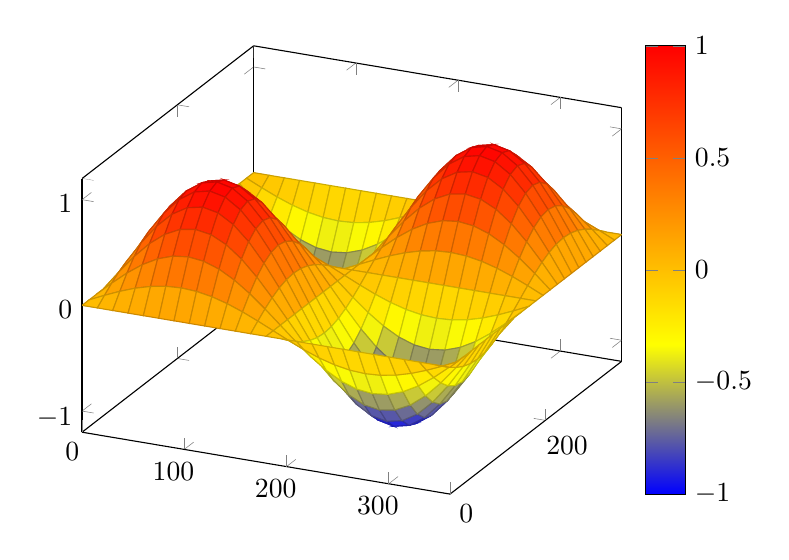
\begin{tikzpicture}
    \begin{axis}[colorbar]
      \addplot3[surf,domain=0:360]
      {sin(x)*sin(y)};
    \end{axis}
  \end{tikzpicture}
  \caption{Représentation graphique de la fonction $f:(x,y)\mapsto
    \sin x\times\sin y$}
  \label{sin-x*sin-y}
\end{figure}

\lipsum[3-10]
%</developpementII-sample|single-sample>
%</these-sample|single-sample|single-template|these-master|developpementII-sample>
%<*these-sample|single-sample|single-template|these-master>
%<<COMMENT
% Sixième chapitre
%COMMENT
%</these-sample|single-sample|single-template|these-master>
%<*these-sample|single-sample|single-template|these-master|conclusionII-sample>
%<single-template>% \chapter{...}
%<single-template>% ...
%<these-master>% \include{corps/}
%<these-sample>\chapter{Conclusion}
%
Dans ce chapitre, nous concluons notre étude.

\lipsum[6-9]

%%% Local Variables: 
%%% mode: latex
%%% TeX-master: "../these"
%%% End: 

%<*conclusionII-sample|single-sample>
\chapter{Conclusion}
Dans ce chapitre, nous concluons l'étude du rire du chaos.

\lipsum[6-9]
%</conclusionII-sample|single-sample>
%</these-sample|single-sample|single-template|these-master|conclusionII-sample>
%<*these-sample|single-sample|single-template|these-master>
%<<COMMENT
%
% Chapitre  de conclusion (générale)
%%%%%%%%%%%%%%%%%%%%%%%%%%%%%%%%%%%%%%%%%%%%%%%%%%%%%%%%%%%%%%%%%%%%%%%%%%%%%%%
%COMMENT
%</these-sample|single-sample|single-template|these-master>
%<*these-sample|single-sample|single-template|these-master|conclusion-master|conclusion-sample>
%<single-template|conclusion-master>\chapter*{Conclusion}
%<single-template|conclusion-master>% ...
%<these-sample|these-master>\chapter*{Conclusion}
% ...


%<*conclusion-sample|single-sample>
\chapter*{Conclusion générale}
\lipsum[26-27]
\section{Une section de conclusion}
\lipsum[28-29]
\subsection{Une sous-section de conclusion}
\lipsum[29-31]
\subsubsection{Une sous-sous-section de conclusion}
\lipsum[31-35]
\paragraph{Un paragraphe de conclusion}
\lipsum[36-38]
\subparagraph{Un sous-paragraphe de conclusion}
\lipsum[39-41]
\subparagraph{Un autre sous-paragraphe de conclusion}
\lipsum[39-41]
\paragraph{Un autre paragraphe de conclusion}
\lipsum[36-38]
\subsubsection{Une autre sous-sous-section de conclusion}
\lipsum[31-37]
\subsection{Une autre sous-section de conclusion}
\lipsum[29-31]
\section{Une autre section de conclusion}
\lipsum[28-43]
%</conclusion-sample|single-sample>
%</these-sample|single-sample|single-template|these-master|conclusion-master|conclusion-sample>
%<*these-sample|single-sample|single-template|these-master>
%<<COMMENT
%
% Liste des références bibliographiques
%COMMENT
%<single-sample|these-sample>\printbibliography
%<single-template|these-master>%\printbibliography
%<<COMMENT
%
%%%%%%%%%%%%%%%%%%%%%%%%%%%%%%%%%%%%%%%%%%%%%%%%%%%%%%%%%%%%%%%%%%%%%%%%%%%%%%%
% Début de la partie annexe éventuelle
%%%%%%%%%%%%%%%%%%%%%%%%%%%%%%%%%%%%%%%%%%%%%%%%%%%%%%%%%%%%%%%%%%%%%%%%%%%%%%%
%COMMENT
%<single-template|these-master>% \appendix
%<these-sample|single-sample>\appendix
%<<COMMENT
%
% Premier chapitre annexe (éventuel)
%COMMENT
%</these-sample|single-sample|single-template|these-master>
%<*single-template|annexe-masterI>
%<<COMMENT
% \chapter{...}
% ...
%COMMENT
%</single-template|annexe-masterI>
%<*these-sample|single-sample|single-template|these-master>
%<these-master>% % \chapter{...}
% ...


%<these-sample>\chapter{Documents juridiques}
\label{chap-juridique}

Cette partie regroupe les documents juridiques officiels.

\section{Licence sous laquelle est publié notre travail}
\label{sec-discours}

\lipsum[11-30]

\section{Transposition de la licence précédente en droit français}
\label{sec-autre-discours}

\lipsum[31-50]

%</these-sample|single-sample|single-template|these-master>
%<*juridique-sample|single-sample>
\chapter{Documents juridiques}
\label{chap-juridique}

Cette partie regroupe les documents juridiques officiels.

\section{Licence sous laquelle est publié notre travail}
\label{sec-discours}

\lipsum[11-30]

\section{Transposition de la licence précédente en droit français}
\label{sec-autre-discours}

\lipsum[31-50]
%</juridique-sample|single-sample>
%<*these-sample|single-sample|single-template|these-master>
%<<COMMENT
% Deuxième chapitre annexe (éventuel)
%COMMENT
%</these-sample|single-sample|single-template|these-master>
%<*single-template|annexe-masterII>
%<<COMMENT
% \chapter{...}
% ...
%COMMENT
%</single-template|annexe-masterII>
%<*these-sample|single-sample|single-template|these-master>
%<these-master>% % \chapter{...}
% ...


%<these-sample>\chapter{Programmes informatiques}
\label{chap-listings}

Les listings suivants sont au cœur de notre travail.

\lstinputlisting[caption={Il est l'heure}]{annexes/programmes/heure.c}
\lstinputlisting[caption={Factorielle}]{annexes/programmes/factorielle.c}

%</these-sample|single-sample|single-template|these-master>
%<*listings-sample|single-sample>
\chapter{Programmes informatiques}
\label{chap-listings}

Les listings suivants sont au cœur de notre travail.

%</listings-sample|single-sample>
%<listings-sample>\lstinputlisting[caption={Il est l'heure}]{annexes/programmes/heure.c}
%<*single-sample|heure-sample>
%<single-sample>\begin{lstlisting}[caption={Il est l'heure}]
#include <stdio.h>
int heures, minutes, secondes;

/****************************************************/
/*                                                  */
/*            print_heure                           */
/*                                                  */
/*   But:                                           */
/*      Imprime l'heure                             */
/*                                                  */
/*   Interface:                                     */
/*      Utilise les variables globales              */
/*           heures, minutes, secondes              */
/*                                                  */
/****************************************************/

void print_heure(void)
{
  printf("Il est %d heure",heures);
  if (heures > 1) printf("s");
  printf(" %d minute",minutes);
  if (minutes > 1) printf("s");
  printf(" %d seconde",secondes);
  if (secondes > 1) printf("s");
  printf("\n");
}
%<single-sample>\end{lstlisting}
%</single-sample|heure-sample>
%<listings-sample>\lstinputlisting[caption={Factorielle}]{annexes/programmes/factorielle.c}
%<*single-sample|factorielle-sample>
%<single-sample>\begin{lstlisting}[caption={Factorielle}]
int factorielle(int n)
{
  if (n > 2) return n * factorielle(n - 1);
  return n;
}
%<single-sample>\end{lstlisting}
%</single-sample|factorielle-sample>
%<*these-sample|single-sample|single-template|these-master>
%<<COMMENT
%
%%%%%%%%%%%%%%%%%%%%%%%%%%%%%%%%%%%%%%%%%%%%%%%%%%%%%%%%%%%%%%%%%%%%%%%%%%%%%%%
% Début de la partie finale
%%%%%%%%%%%%%%%%%%%%%%%%%%%%%%%%%%%%%%%%%%%%%%%%%%%%%%%%%%%%%%%%%%%%%%%%%%%%%%%
%COMMENT
\backmatter
%<<COMMENT
%
% Glossaire (si souhaité distinct de la liste des acronymes). Facultatif.
%COMMENT
%<single-template|these-master>% \printglossary
%<these-sample|single-sample>\printglossary
%<<COMMENT
%
% Index. Facultatif.
%COMMENT
%<single-template|these-master>% \printindex
%<these-sample|single-sample>\printindex
%<<COMMENT
%
% Table des matières
%COMMENT
\tableofcontents
%<<COMMENT
%
% Production de la 4e de couverture. Facultatif.
%COMMENT
\makebackcover
%<<COMMENT
%
%COMMENT
\end{document}
%    \end{macrocode}
%
%    \begin{macrocode}
%</these-sample|single-sample|single-template|these-master>
%    \end{macrocode}
%
%    \begin{macrocode}
%<*bibliography-master>
%</bibliography-master>
%    \end{macrocode}
%
%    \begin{macrocode}
%<*bibliography-sample>
%    \end{macrocode}
%
%    \begin{macrocode}
@Article{	  hp,
  author	= {Poincaré, Henri},
  title		= {Démonstration nouvelle des propriétés de l'indicatrice
		  d'une surface},
  journal	= {Annales de Mathématiques},
  volume	= 13,
  date		= {1874},
  pages		= {449--456}
}

@Book{		  relativite,
  author	= {Einstein, Albert and Lorentz, Hendrik Antoon and
		  Minkowski, Hermann and Weyl, Hermann},
  title		= {The Principle of Relativity},
  publisher	= {Methuen},
  address	= {London},
  date		= {1923}
}

@InBook{	  cond,
  author	= {de Condorcet, Nicolas},
  editor        = {O'Connor, Arhur and Arago, François},
  title		= {Discours prononcé à l'Assemblée Nationale au nom de
                  l'Académie des Sciences à la séance du
                  \formatdate{12}{06}{1790}},
  booktitle	= {Œuvres de Condorcet},
  publisher	= {Firmin Didot Frères},
  address	= {Paris},
  volume	= {1},
  origdate	= {1790-06-12},
  pages         = {508-511},
  url           = {http://gallica.bnf.fr/ark:/12148/bpt6k58105584},
  date  	= {1847}
}

@TechReport{	  unrapport,
  author	= {Nom, Prénom},
  title		= {Titre du rapport technique},
  institution	= {Institution où le rapport a vu le jour},
  date		= {2012}
}

@Manual{	  amsmath,
  title		= {User's Guide for the \textsf{amsmath} Package},
  organization	= {American Mathematical Society},
  date		= {2002-02-25}
}

@PhDThesis{	  knuth63,
  author	= {Knuth, Donald Ervin},
  title		= {Finite semifields and projective planes},
  school	= {California Institute of Technology},
  date		= {1963}
}
%    \end{macrocode}
%
%    \begin{macrocode}
%</bibliography-sample>
%    \end{macrocode}
